\chapter{Design}

\section{Design Philosophy}\label{design-philosophy}

Our design philosophy is simple: follow the user. As often as possible,
we presented our interface concepts to potential users, and allowed
their feedback to guide the design process through the final prototype.

Following a methodology roughly following agile methodologies, we
designed and developed the application collaboratively
(\citet{martin2003agile}). Our process was driven by user experience
design, rather than graphic design. That is, we spent relatively little
time polishing aesthetic interface details, and instead focussed on the
core interactions of the application.

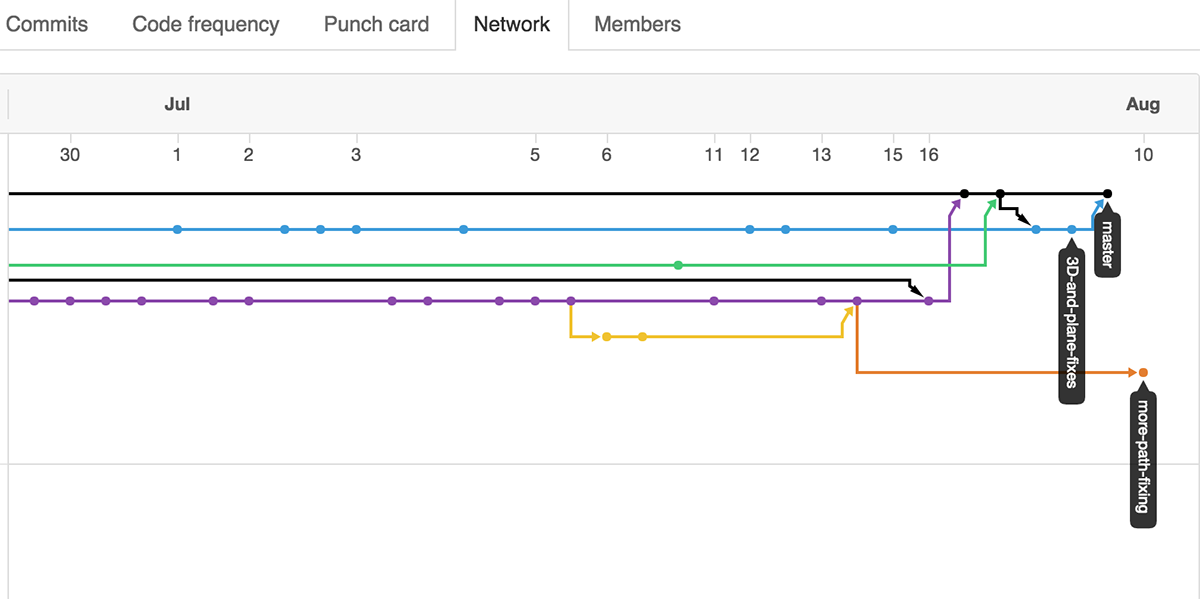
\includegraphics{figures/30_UI_Design_Philosophy/gitflow.png}
\textbf{\textgreater{}\textgreater{}TODO: FIX}

mention affordances of iPad --- cite Gibson/teapot guy. We chose to
design for the iPad as a way of forcing the interface. With a simple,
gesture-based interface, we were forced to

Throughout the design process, we explored the conflict between
creativity and rigid geometric constraints. That is, interfaces that
give the user more room for creative generally tend to make it more
difficult to create designs that will fold correctly in 3D. We aimed for
an interface that provides a great deal of flexibility and creativity,
while guaranteeing that all popup card designs created with it are
valid. Two primary systems maintain this balance.

\begin{enumerate}
\def\labelenumi{\arabic{enumi})}
\itemsep1pt\parskip0pt\parsep0pt
\item
  Tool-based feature creation allows for complex geometry while solving
  geometric constraints transparently.
\item
  The validity system disallows geometry that would interfere with
  existing design elements.
\end{enumerate}

We strive to design an interface that is \textbf{modular},
\textbf{friendly}, and \textbf{delightful}. \textbf{Modularity} stems
from the conception of the pop-up card as a collection of discrete units
that can be acted on individually. Modularity allows users to think in
terms of shape constructions, without concern for individual cuts and
folds. Users can modify, add, and delete individual geometric units,
without modifying the majority of their design. \textbf{Friendliness} is
seen in the careful structuring of our experience to make getting
started as painless as possible. For example, we structure our tutorial
not as a step that must be completed before using the app, but as a
series of brief videos that appear when using a tool for the first time.
\textbf{Delight} comes from small, unexpected details that enhance the
user experience. For example, our color scheme for planes is inspired by
the colors of construction paper. Through this color scheme, we hope to
evoke the spirit of fun and exploration associated with casual
paper-craft.
